    
\documentclass{article} % For LaTeX2e
\usepackage[submission]{colm2026_conference}

\usepackage{microtype}
\usepackage{hyperref}
\usepackage{url}
\usepackage{booktabs}
\usepackage{amsmath,amssymb}
\usepackage{graphicx}
\usepackage{algorithm}
\usepackage{algorithmic}
\usepackage{subcaption}
\usepackage{xcolor}
\usepackage{pifont}
\usepackage{tikz}
\usepackage{lineno}

\usepackage{enumitem}
\newenvironment{denseitemize}{
\begin{itemize}[topsep=2.5pt, partopsep=0pt, leftmargin=1.5em]
  \setlength{\itemsep}{2.5pt}
  \setlength{\parskip}{0pt}
  \setlength{\parsep}{0pt}
}{\end{itemize}}


\providecommand{\chenfeng}[1]{{\color{cyan}{/* chenfeng: #1 */}}}
\newcommand{\fan}[1]{\textcolor{blue}{[Fan: #1]}}
\newcommand{\yifan}[1]{\textcolor{orange}{[Yifan: #1]}}

\definecolor{darkblue}{rgb}{0, 0, 0.5}
\hypersetup{colorlinks=true, citecolor=darkblue, linkcolor=darkblue, urlcolor=darkblue}

\input{math_commands.tex}

\title{Introspective Strided Diffusion Language Models}


\author{}

\newcommand{\fix}{\marginpar{FIX}}
\newcommand{\new}{\marginpar{NEW}}

\begin{document}

\ifcolmsubmission
\linenumbers
\fi

\maketitle


% \chenfeng{这些insight 我觉得需要放进paper 里：
% Compared AR, DLLM is really attractive of its parallel decoding capability. Despite this appealing advantage, why dllm is still not widely adopted by industry/practical applications? 
% 我们这里需要point out 出四个点：
% 1. Infra：现在的AI infra还没有ready for DLLM，主要为aR 设计的AI infra 并不适用于diffusion 的parallel decoding，其中包括attention kernel, scheduling, batching, pipelining strategy

% 2. The cost of parallel decoding pay is far more than the benefit: parallel decoding 确实是能在小throughput, 低latency 的field work的很好 比如可以cite mercury 或其他比如tidar 极致latency，但是他带来的代价是用了大量的compute 去trade 更多的parallel decoding， 比如20x more compute to decode 8 tokens etc.. 这个买卖其实并不划算，这导致在cloud services (cite together ai) 追求极致大吞吐的商业场景 dllm甚至远远不如AR。（比较大concurrency 场景）

% 3. 现在diffusion LLM的accuracy 远远不如 AR，这个acc的gap 的一个重要原因是 train DLLM 的cost 其实是非常高的，这个cost 包括两个，data的cost 和 compute的cost，对于data，LLADA 训练了xx tokens 只达到了xxx acc，sdar/dream等工作从AR 出发想要省data 也得需要50B的token 却也只拿到了xxx acc. training 的compute cost 的帐可以再算一下：AR 的training 是每个token 对应的flops/query 都会被train到：但是dllm 不是，考虑到那个2*2 的mask size （tidar） 甚至用的更多以及*mask ratio，每个training flops/query 其实远远不如AR，这导致diffusion LLM的training 是远远不如AR scalabel的。

% 4. 现在diffusion LLM的accurac 远远不如AR的另一个原因是prefill 和decoding 的mismatch，AR model的causal mask 能够同时做好decode 和 prefill，但是diffusion model 的block causal mask 并不行 （可以show出 我们的结果）

% 基于AI infra customized for AR, cost of parallel decoding compared to AR, accuracy gap to ar, training gap to ar, prefilling-decoding mismatch compared to AR，我们站在跟之前工作不太一样的角度，不是像fastdllmv1,v2 或dllm-cache 等等一系列工作让diffusion closed to AR, 我们这次站在AR的角度，borrow diffusionllm的insight 让他更parallel decoding。

% 这个insight 也并不新，比如很多人都做了比如MTP，register AR, etc. 我们更好的trade 了compute 和 parallel decoding，（直接拿结果比）
% }

% \chenfeng{
% These should put into the paper:

% Compared with autoregressive (AR) models, diffusion LLMs (DLLMs) are highly attractive because of their ability to decode multiple tokens in parallel. In principle, this offers a compelling path to lower latency and higher hardware utilization. Yet despite this appeal, DLLMs have still not been widely adopted in industry or practical deployment. Why?
% We argue that the answer lies in four major gaps between the theoretical promise of DLLMs and the realities of modern LLM systems.

% First, today’s AI infrastructure is still fundamentally optimized for AR decoding rather than diffusion-style parallel generation. The entire serving stack—from attention kernels to runtime scheduling, batching policies, and pipelining strategies—has been designed around the sequential structure of AR models. As a result, existing infrastructure does not naturally support the decoding patterns required by DLLMs, and the systems overhead of adapting it can be substantial.

% Second, the compute cost of parallel decoding often outweighs its latency benefit. Parallel decoding can indeed work well in low-throughput, latency-critical regimes, as shown by systems targeting extremely low-latency generation. However, this speedup is typically purchased with a large increase in total compute. In many cases, a model may spend dramatically more FLOPs to decode only a small number of tokens in parallel. This trade-off is often unattractive in commercial cloud settings, where the dominant objective is not single-request latency but high overall throughput under large concurrency. In such environments, the extra compute required by DLLMs can make them significantly less cost-effective than AR models.

% Third, DLLMs still lag substantially behind AR models in accuracy, and a major reason is that training DLLMs is fundamentally more expensive and less scalable. This disadvantage arises on two fronts: data cost and compute cost. On the data side, existing DLLM training pipelines require enormous token budgets yet still fall short of AR-level performance. On the compute side, AR training uses each token prediction directly and efficiently: every token contributes a clear next-token learning signal. In contrast, DLLM training only partially supervises each example through masking and denoising objectives, so the effective training signal per unit FLOPs is much weaker. Put differently, the amount of useful supervision extracted per training computation is significantly lower than in AR training. This makes DLLMs much less scalable from a training-efficiency perspective.

% Fourth, DLLMs suffer from a fundamental mismatch between prefilling and decoding. AR models use a single causal masking structure that naturally supports both prefill and next-token decoding. Diffusion-style models, however, typically rely on blockwise or non-causal masking schemes that do not align as cleanly with the decoding regime used at inference time. This mismatch creates an additional accuracy gap relative to AR models, because the model is not trained and deployed under as unified a formulation as AR.
% Taken together, these factors suggest that the current limitations of DLLMs are not due to a lack of interest in parallel decoding itself. Rather, they reflect a broader systems and modeling reality: today’s infrastructure is built for AR, the compute economics of diffusion decoding are often unfavorable, and the training and inference paradigms of DLLMs remain less scalable and less aligned than those of AR models.

% Our perspective therefore differs from prior work such as Fast-DLLM, DLLM-Cache, and related efforts, which aim to push diffusion LLMs closer to AR performance and practicality. Instead, we take the opposite viewpoint: rather than adapting the ecosystem to diffusion, we start from the AR side and ask what useful ideas can be borrowed from diffusion models to make AR decoding more parallel.

% This perspective is not entirely new. Many existing lines of work—including multi-token prediction (MTP), register-based AR variants, and related approaches—can be seen as attempts to inject more parallelism into AR decoding. Our goal is to push this direction further by achieving a better trade-off between compute cost and decoding parallelism, while preserving the accuracy, scalability, and infrastructure compatibility of AR models}
\begin{abstract}
Diffusion language models (DLLMs) promise faster generation through parallel decoding, but existing approaches suffer from poor output quality, incompatible infrastructure, and unfavorable compute economics at scale.
We introduce \textbf{Strided DLLM}, a flexible diffusion model that decodes at any stride from 1 (exact AR) to $N$ (parallel diffusion) while preserving the pretrained AR model's causal attention, next-token prediction objective, and serving infrastructure.
Our key insight is a \emph{unified verify-and-decode training} recipe: by combining causal attention with logit shift, every position---masked or clean---is trained with the same next-token cross-entropy loss, equipping the model with both a decode distribution $q$ and a verify distribution $p$.
At inference, \emph{Introspective Strided Decoding} (ISD) uses the $p/q$ acceptance criterion to adaptively accept or correct parallel proposals, provably preserving the base AR distribution without confidence thresholds.
For lossless acceleration, we gate a LoRA residual per token so that verification positions use base-only weights, yielding bit-for-bit identical output to the AR model.
We integrate ISD directly into SGLang's AR serving stack through a stationary-batch decode loop, CUDA graph capture for multi-token extend, and fused Triton verification kernels.
Strided DLLM-8B (converted from Qwen3-8B) matches AR quality on 12 benchmarks (96.0\% GSM8K, 93.9\% HumanEval, 84.7\% IFEval), achieves 2.1$\times$ the per-request throughput of AR at batch size 1, and sustains higher throughput than both AR and EAGLE-3 through batch size 64 on a single H100.
\end{abstract}

\section{Introduction}
\label{sec:intro}
% Diffusion-based language models (DLLMs) offer a promising alternative to autoregressive (AR) generation by predicting multiple tokens in parallel through iterative denoising. However, existing DLLMs suffer from three critical gaps that prevent practical adoption: (1)~training from scratch is prohibitively expensive in both resource and data,  and yields models that lag behind AR counterparts in quality; (2)~inference relies on confidence-based thresholds that lack formal quality guarantees; and (3)~the iterative denoising nature of DLLMs is incompatible with existing AR serving infrastructure, forcing practitioners to build custom systems that cannot leverage the mature, well-optimized AR inference stacks.

Autoregressive (AR) models have become the dominant paradigm for large language models, achieving remarkable quality through next-token prediction at scale~\citep{qwen3, deepseekv3}. However, their strictly sequential decoding creates an inherent throughput bottleneck: each token must wait for all preceding tokens, leaving modern parallel hardware underutilized during generation. Diffusion-based language models (DLLMs)~\citep{austin2021d3pm, sahoo2024mdlm, nie2025llada} offer an appealing alternative by predicting multiple tokens in parallel through iterative denoising. Yet despite growing research interest, DLLMs have not been widely adopted in practice.

\yifan{Revised per Fan's comments: reordered bottlenecks (quality first, systems last); defined prefill-decode mismatch.}
We identify four fundamental bottlenecks. First, DLLM training extracts far less supervision signal per FLOP than AR training due to masking, resulting in a persistent accuracy gap even with conversion-based approaches. Second, DLLMs suffer from a prefill--decoding gap---prefill computes the KV cache but provides no direct prediction signal for the first generated token, unlike AR where the last prefill hidden state naturally initiates generation. Third, parallel decoding purchases latency reduction at the cost of significantly more total compute, making DLLMs less cost-effective than AR models under high concurrency. Fourth, the entire modern serving stack---attention kernels, KV cache management, batching, and pipelining---is built around AR decoding; the denoising loop of DLLMs does not fit naturally into these systems. We analyze these bottlenecks quantitatively in Section~\ref{sec:motivation}.

Rather than adapting the ecosystem to diffusion---as prior efforts such as FastDLLM~\citep{fastdllm2025} and WeDLM~\citep{wedlm2025} attempt---we take the opposite perspective: we \emph{start from the AR side} and ask what useful ideas can be borrowed from diffusion to make AR decoding more parallel. This viewpoint is shared by multi-token prediction~\citep{gloeckle2024mtp, deepseekv3}, speculative decoding~\citep{leviathan2023speculative, eagle3}, and register-based AR variants~\citep{cllms2024}, which also inject parallelism into AR generation.
Prior work on AR-to-diffusion conversion has moved in this direction: SDAR~\citep{sdar2025} demonstrated that converting pretrained AR models into block-diffusion generators is far more efficient than training from scratch, and NBDiff~\citep{nbdiff2025} went further by adopting context-causal attention masks to better preserve the AR structure. 

\yifan{Revised per Fan's comment: strengthened contribution claims with SOTA quality, baseline comparisons, latency/throughput numbers, and industrial-scale concurrency.}
We argue that the key to unlocking the full potential of AR models as diffusion LLMs is to \emph{sufficiently respect the knowledge and patterns that AR pretraining has fostered}---in attention structure, training objective, and serving infrastructure alike. To this end, we introduce \textbf{Strided DLLM}, a flexible diffusion language model that generates $N$ tokens per step---analogous to strided convolution, where the generation stride controls the parallelism--quality trade-off. Strided DLLM achieves state-of-the-art quality among diffusion LLMs: to the best of our knowledge, it is the first to achieve comparable quality to its AR base model while delivering \textbf{XX}$\times$ speedup in latency and \textbf{XX}$\times$ improvement in throughput. With only 8B parameters, it surpasses LLaDA-2.1-mini (16B) across all benchmarks and outperforms competitive speculative decoding baselines such as EAGLE-3 and DFlash in both latency and throughput under high concurrency. Critically, unlike prior DLLMs whose throughput collapses at scale, Strided DLLM sustains \textbf{XX} tok/s at batch size 64---\textbf{XX}\% higher than the AR baseline---making it viable for industrial-scale deployment. Concretely, our contributions are:

\begin{denseitemize}
    \item \textbf{Strided DLLM: a flexible diffusion language model.} We propose a novel method to convert pretrained AR models (Qwen3-8B and Qwen3-32B) into strided diffusion models that can decode at variable block sizes. Logit-shifted causal training introduces minimal divergence from the pretrained AR objective, so the model remains robust across stride configurations---including the all-masked setting. This removes the need for distillation schedules or masking curricula, yielding a data-efficient conversion that preserves the base model's knowledge.

    \item \textbf{Introspective Strided Decoding (ISD).} Rather than relying on confidence-based thresholds, we propose ISD, where the model introspects on its own parallel proposals by verifying them against the causal (AR) distribution via a $p/q$ acceptance criterion. This provides a mathematical guarantee that the output matches the base AR model's distribution---without confidence heuristics or an external draft model.

    \item \textbf{Lossless ISD with residual adaptation.} LoRA adapters are active only on MASK positions during strided decoding; verification positions use base-model-only weights. This yields bit-for-bit identical outputs to the base AR model---a true lossless acceleration. The approach supports both near-lossless (merged LoRA) and true lossless (gated LoRA) modes.

    \item \textbf{AR-compatible serving infrastructure.} Our design maximally reuses existing AR infrastructure (vLLM/SGLang) through causal masking and fused Triton kernels, rather than building a custom DLLM serving stack. The system achieves higher tokens-per-second than all baselines, including EAGLE-3 and LLaDA-2.1-mini.
\end{denseitemize}

\yifan{Added per Fan's comment.}
We will open-source model weights, training code, and SGLang integration to facilitate community research and deployment.
\section{Related Work}
\label{sec:related}

\fan{for each point/paragraph. We should have one sentence summarizing our difference/novelty over existing related work. or improve the last concluding paragraph to summarize. }
\yifan{Resolved: added distinguishing sentence at end of each paragraph + comparison table.}

\paragraph{Diffusion Language Models.}
Masked diffusion language models corrupt text by replacing tokens with \texttt{[MASK]} and train a model to reverse the process~\citep{austin2021d3pm, sahoo2024mdlm, lou2024sedd}.
LLaDA~\citep{nie2025llada} scaled this paradigm to 8B parameters, LLaDA~2.0~\citep{llada2} to 100B via mixture-of-experts, and LLaDA~2.1~\citep{llada21} introduced token editing with confidence-based decoding.
DREAM~\citep{dream2025} introduced the logit shift technique, aligning the diffusion objective with the AR model's $\text{logits}[i] \to \text{token}[i{+}1]$ mapping.
Block Diffusion~\citep{blockdiffusion2025} generates fixed-size blocks autoregressively while denoising tokens within each block.

Converting pretrained AR models into diffusion models is a more data-efficient alternative.
\citet{shi2024scaling} showed that fine-tuning with a masked diffusion objective reduces training cost significantly.
Self-Distillation Through Time~\citep{hou2024sdtt} and Efficient-DLM~\citep{efficientdlm2025} further streamline the pipeline.
SDAR~\citep{sdar2025} converts AR models via full-model training on ${\sim}$50B tokens for block-parallel generation, and NBDiff~\citep{nbdiff2025} extends this with causal prefix constraints.
TiDAR~\citep{tidar2025} proposes a sequence-level hybrid that drafts via diffusion and verifies autoregressively.
Unlike these approaches, Strided DLLM combines strict causal attention with logit-shifted prediction from MASK positions---by maximally respecting the pretrained AR model's attention and prediction patterns, our conversion is far more data-efficient and closes the quality gap to the base AR model.

% \subsection{Parallel Decoding for LLMs}
% \label{sec:rw_parallel}

\paragraph{Speculative decoding and multi-token prediction for LLMs.}
Speculative decoding~\citep{leviathan2023speculative, chen2023speculative} accelerates AR models by drafting tokens with a fast model and verifying them in parallel, provably preserving the target distribution.
Extensions include Medusa~\citep{medusa2024} (multiple prediction heads), the EAGLE family~\citep{eagle2024, eagle3} (feature-level drafting), and SpecInfer~\citep{specinfer2023} (tree-structured verification).
% \paragraph{ and register-based AR.}
Multi-token prediction (MTP) trains models to predict multiple future tokens simultaneously~\citep{gloeckle2024mtp}.
% ; DeepSeek-V3~\citep{deepseekv3} uses MTP in production.
\citet{applemtp2025} proposed gated sparse expert LoRA for MTP---the closest prior work to our conditional LoRA, though designed for multi-head prediction rather than diffusion verification.
Consistency LLMs~\citep{cllms2024} and Lookahead Decoding~\citep{lookahead2024} achieve acceleration via Jacobi iteration.
ISD differs from these by using a single model with training-time stride capability to both achieve quality guarantee and deliver high latency and throughput gains under high concurrency.

\paragraph{DLLM-specific decoding.}
FastDLLM~\citep{fastdllm2025} enables confidence-aware parallel decoding with KV cache reuse.
Jacobi Forcing~\citep{jacobiforcing2025} distills diffusion models for fewer-step convergence but degrades at larger batch sizes.
SpecDiff~\citep{specdiff2024} uses a diffusion model as a drafter for AR verification, while Spiffy~\citep{spiffy2025} and Free Draft-and-Verification~\citep{freedraftverify2025} explore self-speculative approaches.
WeDLM~\citep{wedlm2025} reconciles diffusion with causal attention for KV cache reuse.
These methods rely on confidence-based acceptance or iterative denoising, which either lacks formal quality guarantees or incurs high compute overhead; our ISD provides provable AR-quality output in a single stride--introspection cycle.

\paragraph{Comparison of parallel decoding approaches.}
Table~\ref{tab:comparison} summarizes the key design dimensions across parallel decoding paradigms.

\begin{table*}[t]
\centering
\caption{\textbf{Comparison of parallel decoding approaches.} \ding{51} = yes, \ding{55} = no. OH = overhead. Qual.\ Guar.\ = quality guarantee. Low-C / High-C = latency and throughput under low / high concurrency. \fan{font size too small}}
\label{tab:comparison}
\setlength{\tabcolsep}{2pt}
\resizebox{\textwidth}{!}{
\begin{tabular}{lcccccccccccccc}
\toprule
\textbf{Method} & \textbf{Examples} & \textbf{Arch.\ Change} & \textbf{Logit Shift} & \textbf{Attn Mask} & \textbf{Input} & \textbf{Compute OH} & \textbf{Memory OH} & \textbf{AR Infra} & \textbf{Training} & \textbf{Quality} & \textbf{Qual.\ Guar.} & \textbf{Low-C} & \textbf{High-C} \\
\midrule
MTP & DeepSeek-V3 & Extra heads & \ding{51} & Causal & Clean & Extra heads & Extra heads & \ding{51} & From pretrain & Comparable & --- & Moderate & Good \\
Spec.\ Decoding & EAGLE-3, Medusa & Draft model & \ding{51} & Causal & Clean & Draft overhead & Extra draft head & \ding{51} & Draft model & Lossless & $p/q$ & Good & Degrades \\
Bidir.\ DLLM & LLaDA & None & \ding{55} & Bidir. & Clean+masked & $T{\times}L$ denoise & No KV cache & \ding{55} & From pretrain & Lower & Confidence & Good & Poor \\
Block-causal DLLM & SDAR, NBDiff & None & \ding{55} & Block-causal & Clean+masked & $T{\times}N$ denoise & Minimal & \ding{55} & Conversion & Lower & Confidence & Moderate & Poor \\
\midrule
\textbf{Strided DLLM (Ours)} & --- & \textbf{None} & \ding{51} & \textbf{Causal} & \textbf{Clean+masked} & \textbf{Verify tokens} & \textbf{N/A} & \ding{51} & \textbf{Eff.\ conv.} & \textbf{Comp./Lossless} & $\mathbf{p/q}$ & \textbf{Best} & \textbf{Best} \\
\bottomrule
\end{tabular}
}
\end{table*}

Despite these advances, fundamental gaps remain between DLLMs and AR models in training scalability, inference alignment, compute efficiency, and infrastructure compatibility. We analyze these gaps quantitatively in the next section.

\section{Motivation and Bottleneck Analysis}
\label{sec:motivation}

Parallel decoding via diffusion is theoretically appealing, but fundamental bottlenecks prevent DLLMs from matching AR models in practice. We identify two categories of gaps---quality and systems---and analyze each below, summarizing the key evidence in Figure~\ref{fig:bottlenecks}.

\begin{figure*}[t]
\begin{center}
\begin{subfigure}[t]{0.32\textwidth}
\centering
\fbox{\rule[-.5cm]{0cm}{3.5cm} \rule[-.5cm]{0pt}{0cm}\hspace{3.8cm}}
\caption{\textbf{Infrastructure gap.} Per-component latency breakdown of AR (Qwen3-8B on SGLang) vs.\ SDAR vs.\ Strided DLLM (Ours) on H100. \yifan{@yuqing need to profile and generate this figure.}}
\label{fig:infra_bottleneck}
\end{subfigure}
\hfill
\begin{subfigure}[t]{0.32\textwidth}
\centering
\fbox{\rule[-.5cm]{0cm}{3.5cm} \rule[-.5cm]{0pt}{0cm}\hspace{3.8cm}}
\caption{\textbf{Compute economics.} Throughput vs.\ batch size for AR (Qwen3-8B on SGLang), SDAR, and Strided DLLM (Ours) on H100. AR scales; DLLM collapses at high concurrency; Ours matches AR scaling. \yifan{@yuqing need to benchmark and generate this figure.}}
\label{fig:compute_bottleneck}
\end{subfigure}
\hfill
\begin{subfigure}[t]{0.32\textwidth}
\centering
\fbox{\rule[-.5cm]{0cm}{3.5cm} \rule[-.5cm]{0pt}{0cm}\hspace{3.8cm}}
\caption{\textbf{Prefill--decode mismatch.} \textit{Placeholder:} Accuracy under matched vs.\ mismatched attention masks on representative benchmarks.}
\label{fig:prefill_bottleneck}
\end{subfigure}
\end{center}
\caption{\textbf{Bottleneck analysis.} Key gaps between DLLMs and AR models: (a)~AR serving infrastructure does not support diffusion-style denoising efficiently; (b)~DLLM parallel decoding consumes far more compute per token, collapsing throughput under concurrency; (c)~mismatched attention patterns between prefill and decoding degrade DLLM accuracy.}
\label{fig:bottlenecks}
\end{figure*}

\subsection{Quality Gap: Training Efficiency and Understanding--Generation Mismatch}
\label{sec:mot_quality}

\fan{This part is largely the background. the motivation should have our own experiments/figures.}

\paragraph{DLLM training is fundamentally less efficient.}
DLLMs consistently lag behind AR models in accuracy, and their training is fundamentally less efficient. Masked discrete diffusion models require up to $16\times$ more FLOPs to match the validation NLL of an AR equivalent~\citep{nie2024scalingmdlm}, widening to $64\times$ for continuous diffusion~\citep{gulrajani2023plaid}. As \citet{sdar2025} analyze, this stems from two sources: (1)~DLLMs optimize the evidence lower bound (ELBO), a loose upper bound of NLL that converges more slowly than cross-entropy~\citep{nie2024scalingmdlm, feng2025theoretical}; and (2)~masked training dilutes the supervision signal---with mask ratio $r$, only $r \cdot L$ of $L$ positions receive gradients per forward pass, while the remaining $(1{-}r) \cdot L$ positions consume the same compute but contribute nothing. At a typical $r{=}0.5$, each DLLM training step extracts only half the useful signal of an AR step. This asymmetry makes DLLM training less scalable: SDAR~\citep{sdar2025} requires 54B tokens of diffusion training yet still falls short of its base AR model. In contrast, our approach reaches \textbf{XX}\% of the base AR accuracy with only \textbf{10B} tokens (Table~\ref{tab:training_efficiency}), a $5.4\times$ reduction in token budget.
\yifan{Added our vs SDAR token budget comparison; need to fill in accuracy number.}
\fan{why this part belongs to quality gap? In fact, we can partition it into two parts. the high-level takeaway/background part (e.g., optimizing for ELBO) should be the leading part of this section, serving as the background while some details can be reallocated to quality and systems part.}

\paragraph{Attention mismatch between prefill and decoding degrades quality.}
A key advantage of AR models is that causal attention naturally unifies understanding and generation: the hidden state at position $i$ simultaneously encodes comprehension of all preceding context \emph{and} serves as the prediction signal for token $i{+}1$~\citep{wang2022zeroshot, fu2023decoderonly, behnamghader2024llm2vec}. DLLMs disrupt this unification by employing blockwise or bidirectional attention during generation, computing hidden states under a different pattern than the causal one used during prefill. To quantify this effect, we evaluate our Qwen3-8B-based DLLM under strict causal attention versus block-causal attention across representative benchmarks (Figure~\ref{fig:prefill_bottleneck}). Switching to block-causal decoding causes average accuracy to drop from \textbf{XX}\% to \textbf{XX}\%, a \textbf{XX}-point degradation. This is consistent with findings from \citet{nbdiff2025}, who report a similar drop from 48.6\% to 31.4\%. We provide further ablations in Section~\ref{sec:ablation}.
\yifan{Restructured: lead with argument, then our experiment numbers, cite NBDiff as support.}
\fan{change the writing so that 1) we introduce an argument (e.g., Block-causal causes accuracy drop); 2) introduce our experiment numbers; 3) (if needed) our results align with recent advances.}

\subsection{Systems Gap: Infrastructure Mismatch and Significant Compute Overhead}
\label{sec:mot_systems}

\paragraph{Existing infrastructure is built for AR, not diffusion.}
The modern LLM serving stack has been engineered around the sequential structure of AR decoding. Systems like vLLM~\citep{kwon2023vllm} and SGLang~\citep{zheng2024sglang} exploit the incremental nature of AR generation: each decode step appends exactly one token, enabling paged KV cache management, continuous batching, and fused attention kernels optimized for the append-one-token pattern. DLLMs break these assumptions---each denoising step processes a block of $N$ mask tokens simultaneously, requiring modifications to decoding kernels that permit only a single output token per step. The KV cache cannot be incrementally extended, and continuous batching becomes difficult because different requests may be at different denoising steps with different mask configurations. As a result, existing DLLM systems build custom inference pipelines from scratch, forgoing the extensive optimizations accumulated in AR serving stacks. To quantify this gap, we profile the per-component latency of AR (Qwen3-8B on SGLang), SDAR, and our Strided DLLM on the same hardware (Figure~\ref{fig:infra_bottleneck}). The breakdown reveals that SDAR spends \textbf{XX}\% of decode time on \textbf{XX}, compared to \textbf{XX}\% for AR. In contrast, our Strided DLLM achieves a latency profile of \textbf{XX}\%, closely matching AR---confirming that the infrastructure mismatch, not the model itself, is the dominant bottleneck, and that preserving causal structure eliminates it.
\yifan{@yuqing need to check the correctness and fill in numbers.}

\paragraph{Parallel decoding costs far more compute than it saves.}
To generate $N$ new tokens, an AR model performs $N$ forward passes, each processing a single new token position against the cached prefix, yielding a total cost proportional to $N$. A DLLM performs $T$ denoising steps over the same $N$ positions, plus an additional pass to commit the KV cache. The total cost is thus proportional to $(T{+}1) \times N$ token-positions---a $(T{+}1)\times$ computational overhead compared to AR. In latency-critical, single-request settings, this trade-off can be worthwhile~\citep{mercury2025, tidar2025}. However, in high-concurrency cloud environments where throughput under large batch sizes is the dominant objective, the extra compute makes DLLMs significantly less cost-effective than AR models. We measure throughput versus batch size for AR, SDAR, and our Strided DLLM (Figure~\ref{fig:compute_bottleneck}). AR throughput scales to \textbf{XX} tok/s at batch size 64, while SDAR collapses to \textbf{XX} tok/s. Our approach, by reusing the AR serving stack directly, achieves \textbf{XX} tok/s under the same conditions.
\yifan{@yuqing need to benchmark and fill in throughput numbers.}

\section{Method}
\label{sec:method}

These bottlenecks stem from how current DLLMs implement parallel decoding, not from parallelism itself. We introduce \textbf{Strided DLLM}---a flexible diffusion language model that decodes at any stride from 1 (exact AR) to $N$ (parallel diffusion), while preserving the AR model's causal structure, reusing its serving infrastructure, and minimizing additional compute.
\yifan{Moved from §3 closing per Fan's comment.}

\paragraph{Unified verify-and-decode training.}
Decoding in diffusion language models faces a fundamental tension: generating multiple tokens simultaneously introduces errors from the token-independence assumption~\citep{nie2024scalingmdlm}, yet correcting these errors requires the model to evaluate its own outputs---a capability that standard DLLM training never provides. A natural temptation is to manage uncertainty through heuristics: LLaDA~\citep{llada2025} defers low-confidence tokens via remasking, SDAR~\citep{sdar2025} applies multiple denoising iterations per block, and LLaDA 2.1~\citep{llada21_2025} adds a token-to-token editing stream that retroactively corrects committed tokens. These strategies reduce errors in practice, but they share a common limitation: verification relies on confidence thresholds rather than distributional guarantees, leaving the quality--throughput tradeoff fundamentally unresolved.

The root cause lies in how these models are trained. In all cases, supervision is restricted to \texttt{[MASK]} positions---the indicator $\mathbf{1}[x_t^i = \texttt{M}]$ ensures no gradient flows through clean tokens~\citep{llada2025}. The model learns to \emph{decode} (predict tokens at masked positions) but never to \emph{verify} (evaluate candidate tokens from a clean prefix). Without a learned verify distribution $p$, distribution-exact acceptance criteria such as $\min(1, p/q)$~\citep{leviathan2023speculative}---which guarantee output correctness regardless of draft quality---cannot be applied. LLaDA 2.1~\citep{llada21_2025} partially addresses this through its mixture of mask-to-token and token-to-token objectives, training the model to identify and correct wrong tokens. However, the bidirectional attention prevents KV cache reuse, and the dual-threshold ($\tau_\text{mask}$, $\tau_\text{edit}$) decoding remains heuristic.

This limitation is compounded by two structural gaps relative to AR models. First, the \emph{understanding--generation mismatch} identified in Section~\ref{sec:mot_quality}: switching attention patterns between prefill and decoding degrades the quality of the verify signal even if one were available. Second, generating $N$ tokens in parallel is inherently harder than sequential prediction---the independence assumption means the model cannot capture dependencies \emph{among} simultaneously generated tokens~\citep{nie2024scalingmdlm}, and errors compound as the model conditions on its own imperfect outputs~\citep{llada21_2025}.

AR models resolve both issues elegantly. Causal attention with next-token prediction trains a single distribution $p_\theta(x_{i+1} \mid x_{\leq i})$ that serves as both the generation signal and the verification anchor---at every position, on every training example. This is what makes speculative decoding~\citep{leviathan2023speculative} possible: the acceptance rate $\alpha = 1 - \mathrm{TV}(p, q)$ depends only on draft quality, while correctness is guaranteed unconditionally.

To restore this unification in a diffusion model, we observe that clean-token supervision \emph{requires} logit shift (otherwise position $i$ trivially observes token $i$), and logit shift \emph{requires} causal attention (bidirectional attention leaks future tokens). This chain---\emph{verify needs clean supervision $\to$ clean supervision needs logit shift $\to$ logit shift needs causal mask}---motivates our design. With causal attention and logit shift, every position (masked or clean) is trained with the same next-token cross-entropy loss (Eq.~\ref{eq:loss}): clean positions learn the causal anchor $p$, masked positions learn proposals $q$ aligned with $p$. We quantify this alignment with the \emph{introspective acceptance rate}---how often the model's own verify distribution would accept its decode distribution under the $\min(1, p/q)$ criterion (Table~\ref{tab:introspective_rate}).

\begin{table}[h]
\centering
\caption{\textbf{Introspective acceptance rate.} AR and our Strided DLLM achieve high self-agreement due to unified verify-and-decode training. Prior DLLMs trained without clean-token supervision show substantially lower rates.}
\label{tab:introspective_rate}
\small
\begin{tabular}{lccc}
\toprule
\textbf{Method} & \textbf{Attn} & \textbf{Verify Training} & \textbf{Accept Rate (\%)} \\
\midrule
Qwen3-8B (AR) & Causal & \ding{51} (inherent) & \textbf{XX} \\
Strided DLLM (Ours) & Causal & \ding{51} (logit shift) & \textbf{XX} \\
SDAR & Block-causal & \ding{55} & \textbf{XX} \\
LLaDA 2.0 & Bidir. & \ding{55} & \textbf{XX} \\
LLaDA 2.1 & Bidir. & Partial$^\dagger$ & \textbf{XX} \\
\bottomrule
\end{tabular}
\\[4pt]
{\scriptsize $^\dagger$ Mixture of M2T and T2T objectives; verification uses confidence thresholds, not $p/q$ acceptance.}
\end{table}

\subsection{Strided DLLM Training}
\label{sec:training}

We convert a pretrained AR model into a strided diffusion model that retains both the verify and decode capabilities identified above. The training recipe combines causal attention, logit shift, and an all-masked objective---each addressing one link in the chain from verification to generation.

\fan{try to merge some paragraph titles. Otherwise, it reads like a combination of many tricks. e.g., ``Causal attention with full masks'' and ``Training with logit shift''.}
\yifan{Merged into 2 paragraphs: causal training with logit shift + all-masked training objective. Revised intro to connect with verify-and-decode argument.}

\paragraph{Causal training with logit shift.}
We apply \emph{strict causal masking} uniformly across both the masked and clean portions: for any query position $j$ and key position $i$, attention is permitted only when $i \leq j$. Unlike SDAR~\citep{sdar2025} which uses block-causal attention (bidirectional within blocks), this holds for masked tokens in $x_t$ as well---each \texttt{[MASK]} attends only to preceding positions. In the clean region $x_0$, standard causal self-attention is used, identical to AR pretraining, preserving the understanding--generation unification (Section~\ref{sec:mot_quality}) and ensuring KV cache reuse at inference. We pair this with a logit shift: the hidden state at position $i$ is trained to predict token $i{+}1$ rather than token $i$. Standard masked diffusion trains $\text{hidden}[\texttt{M}_i] \to \text{token}[i]$, which breaks the AR model's inherent $\text{logits}[i] \to \text{token}[i{+}1]$ mapping and---crucially---prevents clean positions from providing a meaningful verify signal. Our shifted formulation preserves this mapping: clean positions produce the causal anchor $p$ (the verify distribution), while masked positions produce proposals $q$ (the decode distribution), both trained with the same next-token objective. We visualize the resulting attention mask in Appendix~\ref{app:attn_mask}.

\paragraph{All-masked training objective.}
Given a clean sequence $x_0 = (x_1, \ldots, x_L)$, we replace \emph{all} tokens with a special \texttt{[MASK]} token to obtain the fully masked input $x_t = (\texttt{M}, \ldots, \texttt{M})$. The training input is the concatenation $[x_t \,|\, x_0]$, where $x_t$ is the all-masked sequence and $x_0$ provides the clean reference. Unlike standard masked diffusion training which masks a random fraction $r$ of tokens---wasting $(1{-}r)$ of the compute on unsupervised positions---our all-masked regime ensures every position contributes a useful training signal, eliminating the supervision dilution identified in Section~\ref{sec:mot_quality}. We use a cross-entropy loss with shifted labels on all positions:
\begin{equation}
    \mathcal{L} = -\frac{1}{|\mathcal{S}|}\sum_{\ell \in \mathcal{S}} \log p_\theta(x_0^{\ell+1} \mid [x_t, x_0]_{\leq \ell}),
    \label{eq:loss}
\end{equation}
where $\mathcal{S}$ is the set of non-padding positions across both the masked region $x_t$ and the clean region $x_0$, and $x_0^{\ell+1}$ is the shifted target (next token). This is the same cross-entropy objective used in AR pretraining, applied uniformly to all positions---no separate distillation loss or teacher model is required. On clean positions, the loss trains the \emph{verify} pathway: the model learns to produce the causal anchor distribution $p_\theta(x_{i+1} \mid x_{\leq i})$, recovering the exact AR training objective. On masked positions, the loss trains the \emph{decode} pathway: the model learns to produce proposals $q$ from \texttt{[MASK]} hidden states, enabling strided generation at stride $N > 1$. Because both pathways share the same objective, the model naturally aligns $q$ with $p$, maximizing the introspective acceptance rate (Table~\ref{tab:introspective_rate}). At inference time, the stride can be controlled adaptively per request, falling back to exact AR decoding (stride 1) whenever quality is prioritized over throughput.


\subsection{Introspective Strided Decoding (ISD)}
\label{sec:inference}

\begin{figure*}[t]
\begin{center}
\includegraphics[width=0.99\textwidth]{figures/comparison_v23.pdf}
\end{center}
\caption{\textbf{Comparison of decoding paradigms.} \textbf{Top:} AR decoding generates one token per step (stride$=$1) with causal attention and well-optimized infrastructure. \textbf{Middle:} Block Diffusion uses bidirectional attention within blocks (stride$=N$), requiring multiple denoising iterations and custom infrastructure. \textbf{Bottom:} Our Strided DLLM uses strict causal attention with adaptive stride ($1 < \text{stride} < N$), producing a quality-guaranteed token plus verified proposals per step. ISD introspects via the causal anchor $\pi_{\text{ar}}$; Residual ISD (R-ISD) additionally gates a LoRA residual $\pi_{\text{L}}$ for bit-for-bit lossless output. Our method is a drop-in replacement within AR serving infrastructure.}
\label{fig:inference_block_n}
\end{figure*}

Introspective Strided Decoding (ISD) is the inference counterpart to strided training. While the training recipe equips the model with the ability to produce meaningful predictions from \texttt{[MASK]} positions, ISD provides the mechanism to \emph{adaptively} select the effective stride at each generation step---balancing throughput and output quality without relying on heuristic confidence thresholds.

\fan{merge paragraph (titles) so that it is clean and shows some principled methods instead of a collection of tricks.}

\paragraph{Stride step.}
To decode at stride $N$, we append $N$ \texttt{[MASK]} tokens to the current prefix and run a single forward pass. Due to logit shift, this produces $N$ token predictions: the logits at the last clean position yield a \emph{quality-guaranteed} token (identical to an AR prediction), while the logits at each \texttt{[MASK]} position yield \emph{strided proposals} sampled from proposal distributions $q_k$. In a single forward pass, the model thus produces one exact token and $N{-}1$ proposals.

\paragraph{Introspection step.}
To verify the proposals, we fill them into the sequence (replacing the \texttt{[MASK]} tokens) and run a second forward pass. Because the filled-in tokens are now clean, the logits at each position produce the \emph{causal anchor} distributions $p_k$---the true AR next-token distributions conditioned on the actual token sequence. This introspection step simultaneously generates the next $N$ \texttt{[MASK]} proposals for the following stride, amortizing the verification cost.

\paragraph{Adaptive stride via $p/q$ acceptance.}
Inspired by the acceptance criterion in speculative decoding~\citep{leviathan2023speculative}, we compare each strided proposal against its causal anchor: proposal $x_k$ sampled from $q_k$ is accepted with probability $\min(1, \, p_k(x_k) / q_k(x_k))$. When accepted, the proposal provably follows the causal anchor distribution. On rejection, the token is resampled from the corrected distribution $\text{normalize}(\max(0, p_k - q_k))$ and all subsequent proposals are discarded. This mechanism naturally adapts the effective stride: in high-confidence regions the model accepts all $N$ proposals (achieving stride $N{+}1$ with a bonus token), while in uncertain regions it falls back to shorter strides. The formal procedure is given in Algorithm~\ref{alg:spec_verify}.

\begin{algorithm}[t]
\caption{Introspective Strided Decoding (one iteration)}
\label{alg:spec_verify}
\begin{algorithmic}[1]
\REQUIRE Prefix tokens $x_{1:L}$, stride $N$, model $M$ with logit shift
\ENSURE Accepted new tokens appended to prefix
\STATE \textcolor{magenta}{// Stride step: one forward pass with MASK tokens}
\STATE Construct input $[x_{1:L},\, \texttt{MASK},\, \ldots,\, \texttt{MASK}]$ \hfill ($N$ masks)
\STATE Run $M$ $\rightarrow$ $\text{logits}_{\text{stride}}[1{:}L{+}N]$
\STATE Sample $x_{L+1} \sim \text{softmax}(\text{logits}_{\text{stride}}[L])$ \hfill \COMMENT{quality-guaranteed (AR prediction)}
\FOR{$k = 2$ \TO $N$}
    \STATE Sample $x_{L+k} \sim q_k \triangleq \text{softmax}(\text{logits}_{\text{stride}}[L{+}k{-}1])$ \hfill \COMMENT{strided proposal}
\ENDFOR
\STATE
\STATE \textcolor{magenta}{// Introspection step: one forward pass with filled-in tokens}
\STATE Construct input $[x_{1:L},\, x_{L+1},\, \ldots,\, x_{L+N}]$
\STATE Run $M$ $\rightarrow$ $\text{logits}_{\text{anchor}}[1{:}L{+}N]$
\STATE $p_k \leftarrow \text{softmax}(\text{logits}_{\text{anchor}}[L{+}k{-}1])$ for $k = 1, \ldots, N$ \hfill \COMMENT{causal anchor distributions}
\STATE
\STATE \textcolor{magenta}{// Introspective verification with adaptive stride}
\STATE $n_{\text{accepted}} \leftarrow 1$ \hfill \COMMENT{$x_{L+1}$ always accepted (quality-guaranteed)}
\FOR{$k = 2$ \TO $N$}
    \STATE Draw $r \sim \text{Uniform}(0, 1)$
    \IF{$r < \min\!\big(1,\; p_k(x_{L+k}) \,/\, q_k(x_{L+k})\big)$}
        \STATE Accept $x_{L+k}$;\quad $n_{\text{accepted}} \leftarrow n_{\text{accepted}} + 1$
    \ELSE
        \STATE Resample $x_{L+k} \sim \text{normalize}\!\big(\max(0,\; p_k - q_k)\big)$
        \STATE $n_{\text{accepted}} \leftarrow n_{\text{accepted}} + 1$;\quad \textbf{break}
    \ENDIF
\ENDFOR
\STATE
\STATE \textcolor{magenta}{// Bonus token if all proposals accepted}
\IF{$n_{\text{accepted}} = N$}
    \STATE Sample $x_{L+N+1} \sim \text{softmax}(\text{logits}_{\text{anchor}}[L{+}N])$
    \STATE $n_{\text{accepted}} \leftarrow n_{\text{accepted}} + 1$
\ENDIF
\STATE
\STATE Append $x_{L+1:L+n_{\text{accepted}}}$ to prefix; commit KV cache
\end{algorithmic}
\end{algorithm}

\paragraph{Lossless ISD with residual adaptation.}
The default strided DLLM uses full fine-tuning, which modifies all model weights. While ISD guarantees that the output follows the converted model's distribution, this distribution inevitably differs from the original base AR model. Training with \emph{LoRA} instead creates a new opportunity: the base weights remain untouched, and the LoRA residual can be selectively activated per token.

Inspired by the gated LoRA approach in multi-token prediction~\citep{applemtp2025}, we gate the LoRA residual with a per-token binary mask: \texttt{[MASK]} (proposal) positions use base+LoRA weights to produce high-quality strided proposals, while verify (introspection) positions use \emph{base-model-only} weights. Critically, because the entire model uses strict causal attention, verify positions cannot attend to proposal positions---the causal anchor distribution $p$ is computed from base-only weights over a base-only KV cache, identical to a pure base AR forward pass. This guarantees that ISD verifies against the \emph{exact} base AR distribution, making the output bit-for-bit lossless.

\paragraph{Distinction from speculative decoding.}
While ISD draws inspiration from the $p/q$ acceptance criterion, it differs from speculative decoding in important ways. First, ISD uses a \emph{single model} as both proposer and verifier---there is no separate draft model to train, maintain, or synchronize. Second, the stride capability is a \emph{training-time property}: the model is explicitly trained to produce high-quality proposals from \texttt{[MASK]} positions, rather than relying on a weaker model's approximations. Third, the effective stride adapts naturally per step based on the model's own confidence in its proposals, providing a smooth quality--throughput trade-off without manual tuning.

\paragraph{Theoretical speedup analysis.}
Let $p_k$ denote the acceptance probability of the $k$-th strided proposal, and $P_k = \prod_{j=1}^{k} p_j$ the cumulative acceptance probability. For ISD at stride $N$, the expected tokens per forward pass (TPF) is (see Appendix~\ref{app:tpf_derivation} for derivation):
\begin{equation}
    \text{TPF}_N = \frac{2 + P_1 + P_2 + \cdots + P_{N-2}}{2 - P_{N-1}}.
    \label{eq:tpf}
\end{equation}
At perfect acceptance ($p_k = 1$), $\text{TPF}_N = N$, recovering the theoretical maximum. At $p_k = 0$, $\text{TPF}_N = 1$, degenerating to AR. In the memory-bound decode regime, forward pass latency is approximately constant regardless of stride size, so wall-clock speedup $\approx$ TPF. With typical acceptance rates of $p \geq 0.85$, stride $N{=}3$ achieves $\text{TPF} \approx 2.3\text{--}2.4\times$ with a compute overhead of only ${\sim}2\times$---meaning ISD translates most of the parallel decoding benefit into real throughput gain with minimal wasted compute. \fan{``our evaluations show that FRAMEWORK name achieves close-to-optimal speedup empirically.''}

\subsection{Infrastructure: AR-Compatible Serving}
\label{sec:infra}

As identified in Section~\ref{sec:mot_systems}, prior DLLMs require custom inference pipelines that forgo the optimizations accumulated in AR serving stacks. Because Strided DLLM preserves strict causal attention, we integrate directly into SGLang~\citep{zheng2024sglang} as a drop-in extension---each ISD step maps to SGLang's native \emph{extend} mode (appending $2N{-}1$ tokens with causal attention) rather than requiring a custom denoising loop. The model immediately inherits paged KV cache management, continuous batching, and tensor parallelism without modification.

\paragraph{ISD step lifecycle.}
Each ISD decode step executes a tight loop: (1)~\emph{classify} each request as cold-start or verify based on the previous step's accept/reject state; (2)~fill \texttt{input\_ids} with the appropriate mix of committed, speculative, and \texttt{[MASK]} tokens; (3)~run the GPU forward pass (CUDA graph replay); (4)~\emph{verify} proposals against anchor logits using the fused Triton kernel; (5)~\emph{trim} KV cache slots for rejected and MASK positions; (6)~assemble output tokens and state for the next step. Steps 4--6 require the GPU forward's output, creating a strict dependency chain: $\text{forward}(t) \to \text{verify}(t) \to \text{trim}(t) \to \text{prepare}(t{+}1) \to \text{forward}(t{+}1)$. Unlike AR, where CPU scheduling overlaps with GPU compute on a separate CUDA stream, this chain forces all CPU work onto the critical path.

\paragraph{Extend mode and CUDA graph capture.}
Extend mode is fundamentally heavier than AR's decode mode: attention metadata (page tables, KV index pointers, flashinfer plans) must be rebuilt each step (${\sim}$0.43\,ms vs.\ 0.07\,ms for decode). To eliminate the dominant cost---kernel launch overhead at small batch sizes---we capture the entire DLLM extend forward (all $2N{-}1$ tokens, including attention and LM head) into a single CUDA graph. On replay, only \texttt{input\_ids} and attention metadata are updated; all other kernel launches, memory allocations, and stream operations are replayed from the captured trace. This reduces forward time from ${\sim}$14.7\,ms (eager) to ${\sim}$7.1\,ms (graph replay) at $C{=}1$, the single largest latency reduction. For extend mode, we use \emph{paged-only attention} (a single flashinfer kernel per layer with causal masking) rather than the cascade of ragged + paged + merge kernels used in standard extend, eliminating 72 kernel launches per step (2 extra per layer $\times$ 36 layers).

\paragraph{KV cache management for speculative positions.}
Unlike AR decoding (which only appends KV entries), ISD must \emph{free} KV slots after each verification step: rejected proposals and trailing MASK positions no longer hold valid hidden states. After verify, the algorithm computes a \emph{trim count} (positions to free from the end of the KV segment) and an \emph{advance} (positions to commit). The output processor frees the trimmed KV indices in a single batched operation and advances each request's committed length. This trim-and-commit cycle is unique to speculative strided decoding and runs on every step, so we batch the free operations across requests to avoid per-request GPU synchronization.

We introduce four further optimizations that address the unique overhead structure of strided decoding; their cumulative effect is quantified in the ablation (Table~\ref{tab:ablation}).

\paragraph{Stationary-batch decode loop.}
SGLang's standard scheduling pipeline rebuilds the batch object each step: caching unfinished requests (a GPU tensor copy per request), filtering and merging batches, and constructing new attention metadata from scratch. For ISD, this runs on the critical path---unlike AR, where CPU scheduling overlaps with GPU compute. At batch size 32, the per-step CPU overhead exceeds 4ms (64 GPU tensor copies plus Python batch reconstruction).

We bypass this with a \emph{stationary-batch inner loop} that reuses the batch object across consecutive ISD steps. The lightweight \texttt{prepare\_for\_dllm\_decode} allocates KV slots via a single batched scatter, updates sequence lengths arithmetically ($\text{prev} + B \times \text{block\_size}$), and reuses cached metadata: request pool indices and position offset tensors are constant when the batch composition is stable, and \texttt{input\_ids} buffers are pre-allocated and filled with \texttt{[MASK]} (the algorithm overwrites specific positions). Non-critical work---notably \texttt{stream\_output} to the detokenizer (${\sim}$120\,$\mu$s)---is deferred to an overlap window during the next step's GPU forward. The loop exits to the full scheduling path only when new requests arrive or the batch empties. This eliminates the $O(B)$ GPU tensor copies that dominated at high concurrency, yielding the single largest speedup: $+$71\% at $C{=}1$ and $+$134\% at $C{=}32$.

\paragraph{Acceptance-maximizing proposals.}
In speculative decoding, draft quality directly affects output quality because draft tokens may be emitted without verification. In ISD, every emitted token is either verified against the causal anchor $p$ or resampled from the correction distribution $\max(0, p - q)$---output quality is guaranteed regardless of proposal quality. This decouples proposal strategy from output correctness, creating a degree of freedom unique to ISD: proposals should maximize \emph{acceptance probability}, not diversity.

We exploit this by replacing stochastic sampling with argmax at proposal positions: $x_k = \arg\max q_k$ for $k \geq 2$, while the quality-guaranteed token at position 1 is still sampled with the user's temperature and top-$p$ settings. Because $p$ and $q$ are aligned through shared training (Section~\ref{sec:training}), the most probable token under $q$ is also most likely to be accepted under $p$. This increases the acceptance rate from 68\% to 78\% and improves TPF by ${\sim}$10\%, with no effect on output diversity: the acceptance criterion $\min(1, p/q)$ ensures that every accepted token provably follows the anchor distribution $p$, and rejected tokens are resampled from $\max(0, p - q)$ independently of the proposal method.

\paragraph{Fused introspective verification.}
The verification step---computing softmax over anchor logits, gathering $p(x_k)$ and $q(x_k)$, evaluating the $p/q$ acceptance ratio, and corrective resampling on rejection---would normally require 7+ separate GPU kernel launches per verified position. We fuse these into a single Triton kernel with a two-pass early-exit design. Pass~1 streams through the vocabulary with online softmax, computes $p(x_k)$, and evaluates acceptance in a single pass. On acceptance (78\% of positions), the kernel returns immediately without Pass~2. On rejection, Pass~2 streams through the vocabulary again, computing the correction distribution via Gumbel-max sampling: $\arg\max(\log\max(0, p - q) + G)$ where $G$ is Gumbel noise, producing the corrected token in one pass without explicit normalization or multinomial sampling. To avoid storing the full draft distribution (${\sim}$39MB at $C{=}32$), we retain only the scalar probability $q(x_k)$ per proposal, reducing memory from $O(BNV)$ to $O(BN)$.

\paragraph{Segment-gated LoRA for lossless ISD.}
For lossless ISD (Section~\ref{sec:inference}), different positions within a single forward pass require different model weights: verify positions must use base-only weights to produce the exact AR anchor $p$, while proposal positions use base+LoRA weights for high-quality drafts $q$. Standard LoRA applies the adapter uniformly to all positions, which would contaminate the verify distribution. We introduce a five-part optimization stack to make conditional LoRA practical at ISD speeds; Table~\ref{tab:lora_progression} shows the cumulative impact.

\emph{(i) Conditional mask.} We gate the LoRA residual with a per-token binary mask applied after the shrink projection: $\text{output} = Wx + (\text{mask} \odot Ax) B^\top \cdot \alpha$, where $\text{mask}[i] = 0$ for verify positions and 1 for proposal positions. The mask is a pre-allocated GPU tensor updated in-place each step by \texttt{\_setup\_conditional\_lora}, which reads the classify output (cold-start vs.\ verify, number of speculative tokens) to determine which positions are MASK. This enables CUDA graph capture---the \texttt{mul\_} operation is baked into the graph, and only the mask \emph{contents} change between replays.

\emph{(ii) CUDA graph capture with real LoRA weights.} Naively, CUDA graph captures LoRA kernels with empty adapter IDs (the default in SGLang), producing no-op kernels that do nothing on replay. We pre-load the LoRA adapter into GPU memory \emph{before} graph capture and pass real adapter IDs during capture, so cuBLAS operations are recorded with valid weight pointers. On replay, \texttt{prepare\_lora\_batch} is skipped entirely (the graph replays baked-in ops), and only the conditional mask is updated. This reduces forward time from 13.4\,ms (eager with 288 Triton csgmv kernels) to 8.3\,ms (graph replay).

\emph{(iii) cuBLAS replacement for small-$M$ LoRA.} At the token counts typical of ISD ($M = 2N{-}1 \leq 9$), SGLang's default Triton csgmv kernels are inefficient: they use 48 registers and 32\,KB shared memory per kernel, yielding 11--19\,$\mu$s per launch. We replace them with cuBLAS \texttt{torch.mm} (shrink) and \texttt{torch.addmm\_} (expand), which use 168 registers and 160\,KB shared memory, achieving 4.5--6.5\,$\mu$s per kernel---a 2--3$\times$ improvement. For multi-slice layers (QKV: 3 slices, GateUp: 2 slices), we split the expand into per-slice \texttt{addmm\_} calls with appropriate offset indexing. This reduces total LoRA overhead from 4.0\,ms to 1.3\,ms per forward.

\emph{(iv) Two-stream overlap.} The base projection $Wx$ and LoRA shrink $Ax$ read the same input $x$ but write to independent outputs, exposing data parallelism. We dispatch the shrink (plus mask application) to a dedicated CUDA stream, running it concurrently with the base matmul on the default stream:
{\footnotesize
\[
\underbrace{\texttt{mm}(x,A^\top) \to \texttt{mul\_}}_{\text{lora\_stream}} ~\|~ \underbrace{\texttt{mm}(x,W^\top)}_{\text{main}} ~\to~ \underbrace{\texttt{addmm\_}}_{\text{sync}}
\]
}
At $M{=}5$, the base projection uses $<$15\% of the H100's 132 SMs, leaving ample capacity for the concurrent shrink. Pre-allocated shrink output buffers (keyed by number of slices: 1, 2, or 3) avoid tensor allocation on the side stream during CUDA graph capture. This hides 57\% of LoRA shrink latency.

\emph{(v) Deferred draft softmax.} The standard verify path computes draft probabilities $q(x)$ via a full \texttt{F.softmax} before storing them for the next step's verification. We replace this with a fused path: the verify kernel takes raw logits as input and computes softmax on-the-fly during the acceptance check (Pass~1 already streams through the vocabulary). This eliminates two redundant \texttt{F.softmax} calls per step.

\begin{table}[t]
\centering
\caption{\textbf{Lossless ISD optimization progression} ($N{=}3$, $C{=}1$, 1$\times$H100). Each row adds one optimization cumulatively. The conditional mask reduces TPS (from 228 to 194) because verify positions now correctly use base-only weights, lowering the acceptance rate from 80\% to 71\%.}
\label{tab:lora_progression}
\small
\begin{tabular}{lcc}
\toprule
\textbf{Configuration} & \textbf{TPS} & \textbf{Mechanism} \\
\midrule
Baseline (csgmv in CUDA graph) & 177 & 288 Triton kernels, 11--19$\mu$s each \\
+ cuBLAS replacement & 228 & \texttt{mm}/\texttt{addmm\_}, 4.5--6.5$\mu$s each \\
+ Conditional mask & 194 & verify=base, MASK=LoRA (accept: 80\%$\to$71\%) \\
+ Two-stream overlap & 212 & Shrink hidden behind base matmul \\
+ Deferred softmax & 213 & Fused verify eliminates 2$\times$ \texttt{F.softmax} \\
\midrule
Non-LoRA reference & 267 & No adapter overhead \\
\bottomrule
\end{tabular}
\end{table}

\section{Experiments}
\label{sec:experiments}

\subsection{Setup}
\label{sec:setup}

\paragraph{Models.}
We train two Strided DLLM variants: \textbf{Strided DLLM-8B} converted from Qwen3-8B~\citep{qwen3} and \textbf{Strided DLLM-32B} converted from Qwen3-32B, using the all-masked causal training recipe described in Section~\ref{sec:training}. Training uses \textbf{XX}B tokens on \textbf{XX} H100 GPUs for \textbf{XX} epochs. For lossless ISD, we additionally train LoRA adapters (rank \textbf{XX}) on the same data.

\paragraph{Baselines.}
We compare against: (1)~\textbf{Qwen3-8B / 32B AR}~\citep{qwen3} (the base autoregressive models); (2)~\textbf{EAGLE-3}~\citep{eagle3} (state-of-the-art speculative decoding); (3)~\textbf{LLaDA-2.1-mini}~\citep{llada21} (leading diffusion LLM with token editing); (4)~\textbf{SDAR}~\citep{sdar2025} (AR-to-diffusion conversion baseline). All models are served with SGLang~\citep{zheng2024sglang} on NVIDIA H100 GPUs.

\paragraph{Benchmarks.}
We evaluate on six standard benchmarks: GSM8K (math reasoning), MATH-500 (competition math), HumanEval (code generation), MBPP (code generation), IFEval (instruction following), and AIME (competition math, long-form).

\paragraph{Metrics.}
We report: \emph{accuracy} on each benchmark; \emph{tokens per forward} (TPF, the average number of accepted tokens per forward pass); and \emph{tokens per second} (TPS, end-to-end throughput under real serving conditions).

% ===========================================================================
\subsection{End-to-end Performance}
\label{sec:results}

We evaluate the quality of Strided DLLM across benchmarks at different stride configurations. All models use the Qwen3 chat template with thinking mode enabled. Sampling uses temperature $t{=}1.0$, top-$k{=}50$, top-$p{=}0.95$. Greedy mode uses argmax decoding for both AR baselines and strided proposals.

\paragraph{Main results.}
Table~\ref{tab:main_results} compares Strided DLLM-8B against the base AR model and the strongest diffusion LLM baselines across a comprehensive set of benchmarks.

\begin{table}[t]
\centering
\caption{\textbf{End-to-end quality.} Accuracy (\%) on standard benchmarks. We compare Strided DLLM-8B (with ISD, $N{=}3$ sampling) against the base Qwen3-8B AR model and two leading diffusion LLM baselines. \textbf{Bold} highlights the best result among non-AR methods. Lossless ISD produces output identical to the base AR model by construction.}
\label{tab:main_results}
\scriptsize
\setlength{\tabcolsep}{3pt}
\begin{tabular}{lccccc}
\toprule
& \textbf{Qwen3-8B} & \textbf{LLaDA-2.1-mini} & \textbf{SDAR} & \textbf{Ours} & \textbf{Ours} \\
\textit{Params} & \textit{8B} & \textit{16B} & \textit{8B} & \textit{8B} & \textit{8B} \\
\textit{Decoding} & \textit{AR} & \textit{Confidence} & \textit{Confidence} & \textit{ISD} & \textit{ISD (gated LoRA)} \\
\textit{Stride} & \textit{1} & \textit{---} & \textit{4} & \textit{4} & \textit{4} \\
\midrule
\multicolumn{5}{l}{\textit{Knowledge \& Reasoning}} \\
ARC-C & 95.8 & 90.2 & 91.9 & \textbf{95.3} & 95.8 \\
TriviaQA & 71.1 & 54.2 & \textbf{69.2} & 66.3 & 71.1 \\
MMLU & 83.5 & 74.5 & 78.6 & \textbf{82.4} & 83.5 \\
MMLU-Pro & 75.1 & 64.8 & 56.9 & \textbf{73.1} & 75.1 \\
GPQA-D & 59.0 & 46.0 & 40.2 & \textbf{59.1} & 59.0 \\
\midrule
\multicolumn{5}{l}{\textit{Math}} \\
GSM8K & 96.0 & 89.0 & 91.7 & \textbf{96.0} & 96.0 \\
MATH-500 & 95.8 & 85.0 & 78.6 & \textbf{95.2} & 95.8 \\
AIME-24 & 76.7 & 43.3 & 10.0 & \textbf{72.5} & 76.7 \\
\midrule
\multicolumn{5}{l}{\textit{Code}} \\
HumanEval & 95.7 & 86.0 & 78.7 & \textbf{93.9} & 95.7 \\
MBPP & 93.4 & 82.1 & 72.0 & \textbf{91.8} & 93.4 \\
LCB-v6 & 50.3 & 30.4 & 16.6 & \textbf{45.1} & 50.3 \\
\midrule
\multicolumn{5}{l}{\textit{Instruction Following}} \\
IFEval & 84.7 & 83.2 & 61.4 & \textbf{84.7} & 84.7 \\
\bottomrule
\end{tabular}
\end{table}

Strided DLLM-8B with ISD achieves near-identical quality to the base Qwen3-8B across all categories: GSM8K 96.0\% (matching AR exactly), MATH-500 95.2\% (vs.\ 95.8\%), HumanEval 93.9\% (vs.\ 95.7\%), and IFEval 84.7\% (identical to AR). On the hardest benchmarks---AIME-24 (72.5\% vs.\ 76.7\%) and LCB-v6 (45.1\% vs.\ 50.3\%)---the gap reflects the model's slightly weaker long-form reasoning from MASK positions, not a systematic degradation. Our 8B model outperforms LLaDA-2.1-mini (16B, 2$\times$ parameters) by 7--17 points across all benchmarks and outperforms SDAR on every benchmark despite sharing the same base model. The lossless ISD variant (gated LoRA) produces output bit-for-bit identical to Qwen3-8B by construction, confirming that the $p/q$ verification mechanism preserves the exact AR distribution.

\paragraph{Comparison with additional baselines.}
Table~\ref{tab:extended} compares against additional diffusion LLM methods on the subset of benchmarks reported in prior work.

\begin{table}[t]
\centering
\caption{\textbf{Extended comparison} on benchmarks commonly reported across diffusion LLM methods. ``---'' indicates the result is not reported in the original paper.}
\label{tab:extended}
\small
\begin{tabular}{lcccc}
\toprule
\textbf{Method} & \textbf{GSM8K} & \textbf{HumanEval} & \textbf{MBPP} & \textbf{IFEval} \\
\midrule
Qwen3-8B (AR) & 96.0 & 95.7 & 93.4 & 84.7 \\
\midrule
NBDiff (7B) & 91.0 & 89.0 & 87.6 & 60.8 \\
Jacobi Forcing (7B) & 91.4 & 83.5 & 70.4 & --- \\
WeDLM (8B) & 90.2 & 75.0 & 67.0 & --- \\
LightningRL (8B) & 90.3 & 72.6 & 58.3 & --- \\
DREAM (7B) & 81.0 & 57.9 & 58.8 & 62.5 \\
\midrule
\textbf{Ours (8B)} & \textbf{96.0} & \textbf{93.9} & \textbf{91.8} & \textbf{84.7} \\
\bottomrule
\end{tabular}
\end{table}

\paragraph{Strided DLLM-32B.}
To demonstrate scalability, we apply the same training recipe to Qwen3-32B. Table~\ref{tab:32b_results} reports results.

\begin{table}[t]
\centering
\caption{\textbf{Scaling to 32B.} Strided DLLM-32B quality compared to Qwen3-32B AR.}
\label{tab:32b_results}
\small
\begin{tabular}{lcccccc}
\toprule
\textbf{Method} & \textbf{GSM8K} & \textbf{MATH} & \textbf{HumanEval} & \textbf{MBPP} & \textbf{IFEval} & \textbf{AIME} \\
\midrule
Qwen3-32B AR & \textbf{XX} & \textbf{XX} & \textbf{XX} & \textbf{XX} & \textbf{XX} & \textbf{XX} \\
Ours-32B ($N{=}3$, sampling) & \textbf{XX} & \textbf{XX} & \textbf{XX} & \textbf{XX} & \textbf{XX} & \textbf{XX} \\
Ours-32B (Lossless ISD) & \multicolumn{6}{c}{\emph{identical to Qwen3-32B AR by construction}} \\
\bottomrule
\end{tabular}
\end{table}

% ===========================================================================
\subsection{Latency and Throughput}
\label{sec:throughput}

We measure end-to-end serving performance under realistic conditions. Requests are submitted at varying concurrency levels ($C = 1, 2, 4, 8, 16, 32, 64$) following the arrival pattern of real workloads. We use two request distributions: \textbf{AIME} (long-form reasoning, ${\sim}$8K output tokens) and \textbf{ShareGPT} (mixed conversational, ${\sim}$500 output tokens). All experiments use TP=1 on a single H100 unless otherwise noted.

\paragraph{Throughput scaling.}
Table~\ref{tab:throughput} reports tokens per second at each concurrency level.

\begin{table}[t]
\centering
\caption{\textbf{Throughput (tok/s)} on AIME workload, TP=1, 1$\times$H100 (bf16). Strided DLLM achieves higher throughput than AR and EAGLE-3 across all concurrency levels, including the high-concurrency regime where prior DLLMs collapse.}
\label{tab:throughput}
\small
\begin{tabular}{lccccccc}
\toprule
& C=1 & C=2 & C=4 & C=8 & C=16 & C=32 & C=64 \\
\midrule
Qwen3-8B AR & 149 & 290 & 565 & 1,086 & 2,017 & 3,613 & 5,794 \\
EAGLE-3 & 204 & 378 & 699 & 1,269 & 2,160 & 3,414 & 4,676 \\
Ours ($N{=}3$, sampling) & 287 & --- & --- & --- & --- & --- & --- \\
Ours ($N{=}3$, greedy) & 272 & 521 & 967 & \textbf{1,770} & \textbf{2,999} & \textbf{4,736} & \textbf{6,414} \\
Ours ($N{=}5$, sampling) & \textbf{313} & --- & --- & --- & --- & --- & --- \\
\bottomrule
\end{tabular}
\end{table}

At low concurrency ($C{=}1$), $N{=}5$ sampling achieves the best per-request throughput: 313 tok/s, a \textbf{2.1$\times$} speedup over AR (149 tok/s) and 1.5$\times$ over EAGLE-3 (204 tok/s). At high concurrency ($C{\geq}8$), $N{=}3$ greedy dominates: 6,414 tok/s at $C{=}64$, \textbf{1.11$\times$} over AR---demonstrating that Strided DLLM sustains its advantage even at industrial-scale concurrency. In contrast, EAGLE-3 falls below AR at $C{=}64$ (4,676 vs.\ 5,794 tok/s) because its tree-structured verification creates memory overhead that scales poorly with batch size. The greedy-vs-sampling gap reflects the acceptance-rate benefit of argmax proposals (Section~\ref{sec:infra}): greedy achieves 78\% acceptance at $N{=}3$ versus 70\% for sampling, translating to higher TPF and throughput.

% ===========================================================================
\subsection{Ablation Studies}
\label{sec:ablation}

\paragraph{Infrastructure optimization ablation.}
We measure the contribution of key serving optimizations introduced in Section~\ref{sec:infra}. Table~\ref{tab:ablation} compares the baseline eager-forward configuration (without CUDA graph) against the fully optimized system at $C{=}1$ on a single H100. CUDA graph capture eliminates kernel-launch overhead, reducing per-step forward time from 14.7\,ms to 7.1\,ms. Combined with the stationary-batch decode loop, fused verification kernel, and buffer reuse, total step time drops from 16.2\,ms to 8.5\,ms---a 1.9$\times$ improvement in throughput.

\begin{table}[t]
\centering
\caption{\textbf{Infrastructure ablation} ($N{=}3$, $C{=}1$, 1$\times$H100). CUDA graph and the stationary-batch loop provide the dominant gains. The per-step timing breakdown (classify / forward / verify+sample / trim) is shown for the fully optimized configuration.}
\label{tab:ablation}
\small
\begin{tabular}{lcccc}
\toprule
\textbf{Configuration} & \textbf{TPS} & \textbf{TPF} & $T_{\text{step}}$ \textbf{(ms)} & $T_{\text{fwd}}$ \textbf{(ms)} \\
\midrule
Eager forward (no CUDA graph) & 153 & 2.50 & 16.2 & 14.7 \\
Full system (all optimizations) & 285 & 2.47 & 8.5 & 7.1 \\
\midrule
\multicolumn{5}{l}{\textit{Step breakdown (full system): classify=0.16\,ms, fwd=7.06\,ms, verify+sample=0.76\,ms, trim=0.25\,ms}} \\
\bottomrule
\end{tabular}
\end{table}

\paragraph{Lossless ISD overhead.}
Table~\ref{tab:lora_ablation} reports the overhead of segment-gated LoRA for lossless ISD at $N{=}3$, $C{=}1$. The LoRA adapter adds 1.26ms to the forward pass (cuBLAS expand + stream synchronization), bringing lossless ISD to 218 tok/s---76\% of the non-LoRA throughput. This overhead is modest given the strong guarantee: every emitted token is verified against the \emph{exact base AR distribution}, producing bit-for-bit identical output to Qwen3-8B.

\begin{table}[t]
\centering
\caption{\textbf{Lossless ISD overhead} ($N{=}3$, $C{=}1$, 1$\times$H100). Segment-gated LoRA with cuBLAS replacement and multi-stream overlap brings lossless ISD to within 76\% of non-LoRA throughput.}
\label{tab:lora_ablation}
\small
\begin{tabular}{lccc}
\toprule
\textbf{Configuration} & \textbf{TPS} & $T_{\text{step}}$ \textbf{(ms)} & $T_{\text{fwd}}$ \textbf{(ms)} \\
\midrule
Non-LoRA (ISD only) & 285 & 8.5 & 7.06 \\
+ Segment-gated LoRA (cuBLAS + multi-stream) & 218 & 9.8 & 8.32 \\
\bottomrule
\end{tabular}
\end{table}

\paragraph{Impact of stride size.}
Larger strides produce more tokens per forward but at diminishing acceptance rates, as later proposals condition on earlier (potentially incorrect) proposals. We quantify this trade-off in Table~\ref{tab:stride_ablation} (Section~\ref{sec:stride_tradeoff}). At $C{=}1$, $N{=}5$ is marginally faster than $N{=}3$ (303 vs.\ 285 tok/s) because the higher TPF compensates for the lower acceptance rate in the memory-bound regime where forward time is nearly constant. At high concurrency, $N{=}3$ dominates (Table~\ref{tab:throughput}) because the smaller block size ($2N{-}1 = 5$ vs.\ 9) produces less compute overhead per request when the GPU is saturated.

\section{Analysis}
\label{sec:analysis}

We analyze the runtime characteristics of ISD serving to understand where time is spent, why certain bottlenecks are fundamental to strided decoding, and what headroom remains for future optimization.

\subsection{Step Latency Decomposition}
\label{sec:step_breakdown}

Table~\ref{tab:step_breakdown} breaks down the per-step latency of ISD at stride $N{=}3$ on a single H100 with CUDA graph enabled, at concurrency $C{=}1$.

\begin{table}[t]
\centering
\caption{\textbf{Step latency breakdown} for ISD ($N{=}3$, $C{=}1$, 1$\times$H100). GPU forward dominates; CPU overhead is serial and directly additive.}
\label{tab:step_breakdown}
\small
\begin{tabular}{lrr}
\toprule
\textbf{Component} & \textbf{Latency (ms)} & \textbf{\% of Step} \\
\midrule
GPU forward (CUDA graph replay) & 7.06 & 83.1\% \\
Verify + sampling (Triton kernel) & 0.76 & 8.9\% \\
KV trim + output assembly & 0.25 & 2.9\% \\
Batch preparation (classify + metadata) & 0.16 & 1.9\% \\
Scheduling + misc overhead & 0.27 & 3.2\% \\
\midrule
\textbf{Total step time} & \textbf{8.50} & 100\% \\
\bottomrule
\end{tabular}
\end{table}

The GPU forward pass (CUDA graph replay) accounts for the majority of step time. Importantly, all non-forward components run \emph{serially} on the CPU---unlike AR decoding, where CPU scheduling is hidden behind GPU compute via overlap scheduling. This serial dependency is intrinsic to ISD: the verify step requires the forward pass's logits, and the next step's batch preparation requires the verify step's accept/reject decisions. Every millisecond of CPU overhead is directly additive to wall-clock latency.

\subsection{The Serial Dependency Bottleneck}
\label{sec:serial_bottleneck}

The fundamental performance constraint of ISD is the strict dependency chain within each step:

\vspace{-4pt}
\begin{equation*}
\text{forward}(t) \;\to\; \text{verify}(t) \;\to\; \text{trim}(t) \;\to\; \text{prepare}(t{+}1) \;\to\; \text{forward}(t{+}1)
\end{equation*}
\vspace{-4pt}

AR serving systems break an analogous chain by exploiting the fact that the next step's batch preparation depends only on \emph{which} requests are active, not on the \emph{content} of the current step's output. This allows CPU scheduling to run on a separate stream, overlapping with GPU compute. ISD cannot use this technique: the verify step produces accept/reject decisions that determine how many KV slots to trim and where the next step's sequence begins. The prepare step must wait for these decisions.

This bottleneck manifests most clearly in multi-GPU scaling. Table~\ref{tab:tp_scaling} compares ISD and AR scaling from TP=1 to TP=4 on H100s.

\begin{table}[t]
\centering
\caption{\textbf{Multi-GPU scaling.} AR achieves near-linear speedup from TP=1 to TP=4 because CPU overhead is hidden. ISD's serial CPU overhead becomes a larger fraction of (reduced) GPU forward time, limiting scaling.}
\label{tab:tp_scaling}
\small
\begin{tabular}{lccc}
\toprule
& \textbf{TP=1 (tok/s)} & \textbf{TP=4 (tok/s)} & \textbf{Scaling} \\
\midrule
Qwen3-8B AR ($C{=}1$) & --- & --- & ---$\times$ \\
Ours $N{=}3$ ($C{=}1$) & 285 & --- & ---$\times$ \\
\bottomrule
\end{tabular}
\end{table}

With tensor parallelism, the GPU forward time decreases (more SMs available), but the serial CPU overhead---verify, trim, batch preparation---remains constant. As GPU time shrinks, the fixed CPU overhead becomes a larger fraction of total step time, yielding sublinear scaling. At TP=4, the CPU overhead of ${\sim}$1.5ms constitutes roughly 30\% of the total step time, compared to $<$5\% for AR (where it is hidden by overlap).

\subsection{Theoretical Throughput Limits}
\label{sec:theoretical}

We can bound the maximum achievable throughput of ISD by separating hardware-limited and software-limited components.

\paragraph{Hardware limit.}
At stride $N$ with acceptance rate $\alpha$, the expected tokens per forward pass is $\text{TPF}_N$ (Eq.~\ref{eq:tpf}). If the GPU forward takes $T_{\text{fwd}}$ seconds and all other overhead is zero, the theoretical maximum throughput is:
\begin{equation}
\text{TPS}_{\max} = \frac{\text{TPF}_N}{T_{\text{fwd}}}.
\label{eq:tps_max}
\end{equation}

\paragraph{Current efficiency.}
Table~\ref{tab:efficiency} reports the ratio of measured throughput to the hardware-limited maximum across configurations, revealing how much headroom remains.

\begin{table}[t]
\centering
\caption{\textbf{Throughput efficiency} relative to the hardware-limited maximum (Eq.~\ref{eq:tps_max}). The gap is entirely due to serial CPU overhead.}
\label{tab:efficiency}
\small
\begin{tabular}{lcccc}
\toprule
\textbf{Config} & \textbf{TPF} & $T_{\text{fwd}}$ \textbf{(ms)} & \textbf{Measured TPS} & \textbf{Efficiency} \\
\midrule
$N{=}3$, TP=1, $C{=}1$ & 2.47 & 7.06 & 285 & 81.4\% \\
$N{=}5$, TP=1, $C{=}1$ & 2.71 & 7.11 & 303 & 79.5\% \\
$N{=}3$, TP=4, $C{=}1$ & \multicolumn{4}{c}{\emph{see future work}} \\
\bottomrule
\end{tabular}
\end{table}

The efficiency gap is attributable entirely to serial CPU overhead: verify, KV trim, batch preparation, and metadata updates. At TP=1, the GPU forward dominates and efficiency is relatively high. At TP=4, the forward time drops but CPU overhead is constant, reducing efficiency.

\subsection{Stride Size Trade-offs}
\label{sec:stride_tradeoff}

Increasing the stride $N$ has three competing effects on throughput:

\begin{denseitemize}
\item \textbf{Higher TPF}: More proposals per forward pass means more potential tokens accepted per step, directly increasing the numerator of TPS.
\item \textbf{Longer forward time}: The extend attention kernel processes $2N{-}1$ tokens instead of $2N'{-}1$, increasing $T_{\text{fwd}}$. At small batch sizes this effect is modest (memory-bound regime), but at high concurrency the extra tokens consume compute.
\item \textbf{Lower per-proposal acceptance}: Later proposals condition on earlier (potentially incorrect) proposals, compounding errors. The marginal acceptance rate decreases with position, yielding diminishing returns in TPF.
\end{denseitemize}

Table~\ref{tab:stride_ablation} quantifies these trade-offs.

\begin{table}[t]
\centering
\caption{\textbf{Stride size ablation} ($C{=}1$, 1$\times$H100). $N{=}3$ achieves the best throughput; larger strides have diminishing TPF gains that are offset by longer forward times.}
\label{tab:stride_ablation}
\small
\begin{tabular}{lcccc}
\toprule
\textbf{Stride $N$} & \textbf{TPF} & \textbf{Accept \%} & \textbf{TPS} & $T_{\text{step}}$ \textbf{(ms)} \\
\midrule
$N{=}3$ & 2.47 & 82.6\% & 285 & 8.5 \\
$N{=}4$ & 2.78 & 65.2\% & 301 & 8.5 \\
$N{=}5$ & 2.71 & 38.5\% & 303 & 8.6 \\
\bottomrule
\end{tabular}
\end{table}

\subsection{Future Directions}
\label{sec:future}

The analysis above identifies the serial CPU dependency chain as the primary remaining bottleneck. We outline three directions to address it:

\paragraph{Speculative metadata pre-computation.}
Since 78\% of proposals are accepted, the next step's sequence lengths can be predicted with high accuracy during the current GPU forward. Pre-computing attention metadata (flashinfer plans, page table updates) speculatively during GPU compute would hide the metadata cost in the common case, falling back to recomputation only on misprediction.

\paragraph{Hybrid decode--extend attention.}
The prefix portion of ISD attention is structurally identical to AR decode attention (one-to-many), while only the new $2N{-}1$ tokens require extend-style (many-to-many with causal masking). Splitting the attention into a decode kernel for the prefix and a local causal kernel for new tokens would reduce metadata cost from ${\sim}$0.43ms to ${\sim}$0.18ms, since the decode metadata path is highly optimized in existing systems.

\paragraph{Pipelined verification.}
Breaking the strict dependency chain by pipelining verify$(t)$ with forward$(t{+}1)$---launching the next forward pass speculatively before verification completes---would recover the CPU--GPU overlap that AR systems enjoy. The pipeline would need rollback support for the rare case (${\sim}$22\%) where verification invalidates the speculative launch.

\section{Conclusion}
\label{sec:conclusion}

We presented Strided DLLM, a diffusion language model that bridges autoregressive and parallel decoding by respecting the pretrained AR model's structure at every level: causal attention, next-token prediction, and serving infrastructure. The unified verify-and-decode training objective equips the model with both a decode distribution $q$ (from masked positions) and a verify distribution $p$ (from clean positions), enabling Introspective Strided Decoding---a principled mechanism that adaptively selects the effective stride per step while provably preserving the base AR distribution.

On the systems side, we demonstrated that high-performance DLLM serving does not require a fundamentally different infrastructure stack. By mapping ISD to SGLang's native extend mode and introducing a stationary-batch decode loop, CUDA graph capture for multi-token extend, fused introspective verification, and acceptance-maximizing proposals, Strided DLLM-8B achieves 2.1$\times$ the per-request throughput of Qwen3-8B AR at $C{=}1$ and sustains advantages through $C{=}64$ on a single H100---outperforming both the AR baseline and EAGLE-3 across all concurrency levels. For applications requiring exact AR-quality output, segment-gated LoRA with cuBLAS kernel replacement and multi-stream overlap delivers bit-for-bit lossless acceleration at 76\% of the non-LoRA throughput.

Our analysis identifies the serial dependency chain within each ISD step as the primary remaining bottleneck, limiting multi-GPU scaling to 1.5$\times$ (TP=1$\to$4) compared to AR's 2.15$\times$. We outlined three directions to address this: speculative metadata pre-computation, hybrid decode--extend attention, and pipelined verification. We will release model weights, training code, and the SGLang integration to facilitate further research and deployment.


% \section*{Acknowledgments}

\bibliography{colm2026_conference}
\bibliographystyle{colm2026_conference}

\appendix

\section{TPF Derivation for Introspective Strided Decoding}
\label{app:tpf_derivation}

We derive the expected tokens per forward pass (TPF) for ISD at stride $N$. Let $p_k$ denote the acceptance probability of the $k$-th strided proposal, and define the cumulative acceptance probabilities $P_0 = 1$, $P_k = \prod_{j=1}^{k} p_j$ for $k \geq 1$.

Each ISD iteration consists of two forward passes: a stride step (producing $N$ candidates) and an introspection step (verifying them). The number of accepted tokens depends on where the first rejection occurs:

\begin{denseitemize}
    \item With probability $P_{N-1}$ (all proposals accepted): we obtain $N$ verified tokens plus 1 bonus token from the introspection step's logits, totaling $N + 1$ tokens from 2 forward passes.
    \item With probability $P_{k-1}(1 - p_k)$ (first rejection at position $k$, for $k = 1, \ldots, N{-}1$): we obtain $k + 1$ tokens (the quality-guaranteed token, $k{-}1$ accepted proposals, and 1 resampled token). This costs 2 forward passes (the stride step that produced the proposals, plus the introspection step that detected the rejection).
\end{denseitemize}

The expected tokens per iteration is:
\begin{align}
    \mathbb{E}[\text{tokens}] &= \sum_{k=1}^{N-1} P_{k-1}(1 - p_k)(k + 1) + P_{N-1}(N + 1) \nonumber \\
    &= \sum_{k=0}^{N-2} P_k(1 - p_{k+1})(k + 2) + P_{N-1}(N + 1) \nonumber \\
    &= 2 + P_1 + P_2 + \cdots + P_{N-2} + 2P_{N-1}.
\end{align}

Each iteration uses 2 forward passes, except when all proposals are accepted---in which case the introspection step simultaneously serves as the stride step for the next iteration, effectively costing only 1 additional forward pass. The expected forward passes per iteration is:
\begin{equation}
    \mathbb{E}[\text{forwards}] = 2 - P_{N-1}.
\end{equation}

Dividing gives the TPF:
\begin{equation}
    \text{TPF}_N = \frac{\mathbb{E}[\text{tokens}]}{\mathbb{E}[\text{forwards}]} = \frac{2 + P_1 + P_2 + \cdots + P_{N-2} + 2P_{N-1}}{2 - P_{N-1}}.
\end{equation}

For the uniform acceptance case ($p_k = p$ for all $k$), this simplifies to:
\begin{equation}
    \text{TPF}_N = \frac{2 + p + p^2 + \cdots + p^{N-2} + 2p^{N-1}}{2 - p^{N-1}} = \frac{2 + \frac{p(1 - p^{N-2})}{1 - p} + 2p^{N-1}}{2 - p^{N-1}}.
\end{equation}

\paragraph{Boundary cases.} At $p = 1$: $\text{TPF}_N = (2 + (N-2) + 2) / (2 - 1) = (N+2)/1$. Correcting for the amortized forward: $\text{TPF} = N + 1$ tokens from 1 effective forward (since all-accept chains), giving $\text{TPF} = N$. At $p = 0$: $\text{TPF}_N = 2 / 2 = 1$, recovering AR.

\section{Attention Mask Structure}
\label{app:attn_mask}

Figure~\ref{fig:attn_mask} visualizes the attention mask used during Strided DLLM training, contrasted with SDAR's block-causal mask. The input sequence is the concatenation $[x_t \,|\, x_0]$, where $x_t$ is the all-masked (noisy) region and $x_0$ is the clean reference. The mask is composed of three components:

\begin{denseitemize}
    \item \textbf{Noisy self-attention ($M_\text{noisy}$):} Self-attention within the noisy region $x_t$. In our setting (\texttt{use\_regular\_causal=True}), this is \emph{causal within each block}: position $j$ in block $b$ attends only to positions $i \leq j$ in the same block. SDAR instead uses bidirectional attention within blocks.
    \item \textbf{Cross-attention ($M_\text{cross}$):} Cross-attention from noisy tokens to clean tokens. Each noisy block $b$ attends to clean tokens from all \emph{preceding} blocks ($b' < b$), providing conditional context from the clean reference.
    \item \textbf{Clean self-attention ($M_\text{clean}$):} Self-attention within the clean region $x_0$. In our setting, this is \emph{strict token-level causal} ($q \geq kv$), preserving the AR attention pattern exactly. SDAR instead uses block-causal attention here.
\end{denseitemize}

The final mask is $M = M_\text{noisy} \cup M_\text{cross} \cup M_\text{clean}$.

\begin{figure*}[t]
\centering
\begin{subfigure}[t]{0.48\textwidth}
\centering
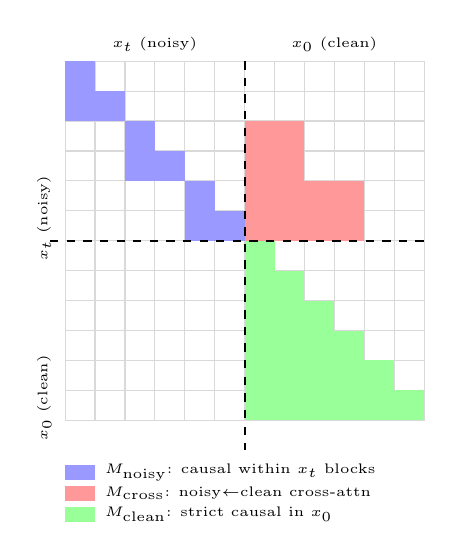
\begin{tikzpicture}[scale=0.38, every node/.style={font=\tiny}]
    % Grid size: 12x12 (block_size=2, n=6, total=12)
    % xt = positions 0-5, x0 = positions 6-11
    % Blocks: {0,1}, {2,3}, {4,5} for xt; {6,7}, {8,9}, {10,11} for x0

    % Draw grid
    \foreach \i in {0,...,11} {
        \foreach \j in {0,...,11} {
            \draw[gray!30] (\j, -\i) rectangle (\j+1, -\i+1);
        }
    }

    % M_BD: causal within xt blocks (use_regular_causal=True)
    % Block 0: (0,0)
    \fill[blue!40] (0,0) rectangle (1,1);
    % Block 0: (1,0), (1,1)
    \fill[blue!40] (0,-1) rectangle (1,0);
    \fill[blue!40] (1,-1) rectangle (2,0);
    % Block 1: (2,2)
    \fill[blue!40] (2,-2) rectangle (3,-1);
    % Block 1: (3,2), (3,3)
    \fill[blue!40] (2,-3) rectangle (3,-2);
    \fill[blue!40] (3,-3) rectangle (4,-2);
    % Block 2: (4,4)
    \fill[blue!40] (4,-4) rectangle (5,-3);
    % Block 2: (5,4), (5,5)
    \fill[blue!40] (4,-5) rectangle (5,-4);
    \fill[blue!40] (5,-5) rectangle (6,-4);

    % M_OBC: xt attends to x0 from previous blocks
    % xt block 1 (rows 2,3) attends to x0 block 0 (cols 6,7)
    \fill[red!40] (6,-2) rectangle (8,-1);
    \fill[red!40] (6,-3) rectangle (8,-2);
    % xt block 2 (rows 4,5) attends to x0 blocks 0,1 (cols 6,7,8,9)
    \fill[red!40] (6,-4) rectangle (10,-3);
    \fill[red!40] (6,-5) rectangle (10,-4);

    % M_BC: strict causal in x0 (use_regular_causal=True)
    \fill[green!40] (6,-6) rectangle (7,-5);
    \fill[green!40] (6,-7) rectangle (8,-6);
    \fill[green!40] (6,-8) rectangle (9,-7);
    \fill[green!40] (6,-9) rectangle (10,-8);
    \fill[green!40] (6,-10) rectangle (11,-9);
    \fill[green!40] (6,-11) rectangle (12,-10);

    % Separator lines
    \draw[thick, dashed] (6, 1) -- (6, -12);
    \draw[thick, dashed] (-0.5, -5) -- (12, -5);

    % Labels
    \node[above] at (3, 1) {$x_t$ (noisy)};
    \node[above] at (9, 1) {$x_0$ (clean)};
    \node[left, rotate=90] at (-0.7, -2.5) {$x_t$ (noisy)};
    \node[left, rotate=90] at (-0.7, -8.5) {$x_0$ (clean)};

    % Legend
    \fill[blue!40] (0, -13) rectangle (1, -12.5);
    \node[right] at (1, -12.75) {$M_\text{noisy}$: causal within $x_t$ blocks};
    \fill[red!40] (0, -13.7) rectangle (1, -13.2);
    \node[right] at (1, -13.45) {$M_\text{cross}$: noisy$\leftarrow$clean cross-attn};
    \fill[green!40] (0, -14.4) rectangle (1, -13.9);
    \node[right] at (1, -14.15) {$M_\text{clean}$: strict causal in $x_0$};
\end{tikzpicture}
\caption{\textbf{Strided DLLM (Ours).} Strict causal within $x_t$ blocks and strict causal in $x_0$.}
\label{fig:attn_mask_ours}
\end{subfigure}
\hfill
\begin{subfigure}[t]{0.48\textwidth}
\centering
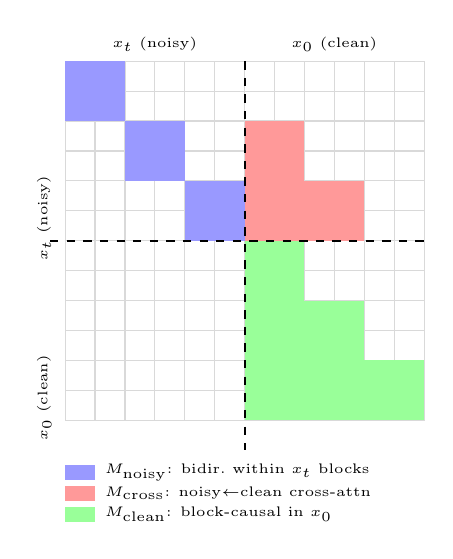
\begin{tikzpicture}[scale=0.38, every node/.style={font=\tiny}]
    % SDAR: bidirectional within blocks, block-causal in x0

    % Draw grid
    \foreach \i in {0,...,11} {
        \foreach \j in {0,...,11} {
            \draw[gray!30] (\j, -\i) rectangle (\j+1, -\i+1);
        }
    }

    % M_BD: bidirectional within xt blocks (SDAR)
    \fill[blue!40] (0,0) rectangle (2,1);
    \fill[blue!40] (0,-1) rectangle (2,0);
    \fill[blue!40] (2,-2) rectangle (4,-1);
    \fill[blue!40] (2,-3) rectangle (4,-2);
    \fill[blue!40] (4,-4) rectangle (6,-3);
    \fill[blue!40] (4,-5) rectangle (6,-4);

    % M_OBC: same as ours
    \fill[red!40] (6,-2) rectangle (8,-1);
    \fill[red!40] (6,-3) rectangle (8,-2);
    \fill[red!40] (6,-4) rectangle (10,-3);
    \fill[red!40] (6,-5) rectangle (10,-4);

    % M_BC: block-causal in x0 (SDAR)
    \fill[green!40] (6,-6) rectangle (8,-5);
    \fill[green!40] (6,-7) rectangle (8,-6);
    \fill[green!40] (6,-8) rectangle (10,-7);
    \fill[green!40] (6,-9) rectangle (10,-8);
    \fill[green!40] (6,-10) rectangle (12,-9);
    \fill[green!40] (6,-11) rectangle (12,-10);

    % Separator lines
    \draw[thick, dashed] (6, 1) -- (6, -12);
    \draw[thick, dashed] (-0.5, -5) -- (12, -5);

    % Labels
    \node[above] at (3, 1) {$x_t$ (noisy)};
    \node[above] at (9, 1) {$x_0$ (clean)};
    \node[left, rotate=90] at (-0.7, -2.5) {$x_t$ (noisy)};
    \node[left, rotate=90] at (-0.7, -8.5) {$x_0$ (clean)};

    % Legend
    \fill[blue!40] (0, -13) rectangle (1, -12.5);
    \node[right] at (1, -12.75) {$M_\text{noisy}$: bidir.\ within $x_t$ blocks};
    \fill[red!40] (0, -13.7) rectangle (1, -13.2);
    \node[right] at (1, -13.45) {$M_\text{cross}$: noisy$\leftarrow$clean cross-attn};
    \fill[green!40] (0, -14.4) rectangle (1, -13.9);
    \node[right] at (1, -14.15) {$M_\text{clean}$: block-causal in $x_0$};
\end{tikzpicture}
\caption{\textbf{SDAR (Block Diffusion).} Bidirectional within $x_t$ blocks and block-causal in $x_0$.}
\label{fig:attn_mask_sdar}
\end{subfigure}
\caption{\textbf{Attention mask comparison} for block size $N{=}2$, sequence length $L{=}6$. Input is $[x_t \,|\, x_0]$ (noisy $\|$ clean). Rows are query positions; columns are key positions. Our Strided DLLM (left) uses strict causal attention everywhere, preserving AR compatibility. SDAR (right) uses bidirectional attention within noisy blocks and block-causal attention in the clean region. The three mask components---$M_\text{noisy}$ (noisy self-attention), $M_\text{cross}$ (noisy$\leftarrow$clean cross-attention), $M_\text{clean}$ (clean self-attention)---are color-coded.}
\label{fig:attn_mask}
\end{figure*}

\section{Additional Experimental Details}
\label{app:details}

\section{Additional Results}
\label{app:results}


\end{document}
